\chapter{涂鸦线标签下基于图相似度传播的弱监督语义分割}
\label{chp:scribble}
\section{引言}
% 涂鸦线标签
弱监督语义分割可以由形式各异的多种视觉标签所驱动,不同种类的标签能够为模型训练提供不同量级的信息量,进而得到不同精度水平的语义分割模型。
其中,涂鸦线标签作为一种简单而又直观的监督标注形式,指的是标注者直接在目标上方绘制一条不规则的涂鸦线条,用于标识该目标的大致位置和所属类别。
\figureref{fig:scribble-samples}展示了 PASCAL VOC 2012 数据集中三幅图片及它们的涂鸦线标签,其中不同颜色的线条对应不同的目标类别。
\par
\begin{figure}[h]
\centering
\subfloat[]{\includegraphics[width=.3\linewidth]{scribble-sample-1}%
\label{subfig:scribble-sample-1}}
\hfil
\subfloat[]{\includegraphics[width=.3\linewidth]{scribble-sample-2}%
\label{subfig:scribble-sample-2}}
\hfil
\subfloat[]{\includegraphics[width=.3\linewidth]{scribble-sample-3}%
\label{subfig:scribble-sample-3}}
\caption{涂鸦线标签示例}
\label{fig:scribble-samples}
\end{figure}
\par
% 涂鸦线标签的优势
% 点标签可以视为线标签的一种特殊情况,成本相近但能提供非常多额外的信息
相比于图片级的分类标签,涂鸦线标签能够表征出目标的大致位置,对于检测、分割等任务较有帮助。
相比于像素级的分割标签,涂鸦线标签仅要求标注者在目标上随意画线,无需精准标出目标的所有像素,极大降低了标注成本。
另外,涂鸦线标签与目标检测任务中的边界框标签具有相近的标注成本,后者仅给出目标的外接矩形,所框定范围并不都是目标像素点,而前者能够提供完全可信的目标像素点,更有利于分割这种像素级任务的训练。
尽管涂鸦线标签相比于其他标签有诸多优势,目前在实际应用时,线监督的语义分割仍然存在以下两个难点:
\par
% 涂鸦线标签的难点
(1)\textbf{标注存在主观性}:
这是与传统的分类、检测、分割标签最大的不同点。
对于涂鸦线标签,我们仅要求标注者在目标上方随意画一条线。
尽管线的粗细可以预设,但其出现位置和覆盖范围都存在很大的随机性。
对于同一个目标,不同标注者,甚至是同一标注者在不同时间,都会画出完全不一样的标签。
这种标注主观性将影响到用于训练的伪标签的质量,最终降低训练得到的语义分割网络的精度。
\par
(2)\textbf{缺失边缘先验}:
大多数情况下,标注者都会选择在目标的中心区域画线,而不会仔细刻画出目标的轮廓(否则就失去了涂鸦线作为弱标签的低成本优势)。
此时,单纯从涂鸦线标签无法直接获得目标的边缘先验,只能获知目标中心大致有哪些像素,却不知道这些像素的边界在哪里。
相比之下,框标签虽然也没有直接刻画目标的精确轮廓,但对归属于目标的像素点做了范围限制,一定程度上比线标签更有利于定位边缘。
这种边缘先验的缺失对于边缘检测、语义分割、实例分割等像素级任务较为不利,通常要求模型设计额外的模块(如 CRF\cite{krahenbuhl2011efficient})来补全边缘信息。
\par
% 难点解决
为了解决以上这些问题,本章节以涂鸦线标签为研究对象,设计了一种面向自然图像的、基于图相似度传播的弱监督语义分割框架 GAP-CAM。
该框架首先设计了一种基于视觉注意力图的伪标签初始化策略,借助于分类标签不随标注者而变化的特点,规避了线标签的主观性对于模型性能的影响;然后,基于超像素与图卷积算子设计了一个区域相似度建模网络,最后
\section{基于图相似度传播的自然图像弱监督分割框架 GAP-CAM}\label{sec:gapcam}
\begin{figure}[h]
\centering
\includegraphics[width=\linewidth]{gapcam-arch}
\caption{基于图相似度传播的弱监督语义分割框架 GAP-CAM}
\label{fig:gapcam-arch}
\end{figure}
% 对框架 GAP-CAM 的一段话介绍
GAP-CAM(\textbf{G}raph \textbf{A}ffinity \textbf{P}ropagation - \textbf{C}lass \textbf{A}ctivation \textbf{M}ap)
\subsection{基于视觉注意力图的伪标签初始化策略}
\label{subsec:cam}
直观来看,一个图像分类网络使用类别标签进行训练,输出不带空间信息的类别概率向量,理论上无法提供任何关于目标位置或目标大小的额外信息。
随着神经网络可解释性领域的发展,研究者指出,分类网络对目标在空间中的位置有相当的感知能力,从面向分类的卷积神经网络中提取出目标的粗略定位信息是可行的,能够用于解释其分类结果\cite{oquab2015object}。
亦即,通过一定的结构设计,我们能够用图像级的类别标签训练出具有定位能力的神经网络。
这启示我们,针对涂鸦线监督的语义分割,可以先将涂鸦线标签转换为完备的类别标签,训练得到分类网络,提取网络中蕴涵的目标位置信息,用于辅助弱监督学习中伪标签的初始化,为后续分割网络的训练作好准备。
\par
目前,针对图像分类模型在目标定位方面的研究主要分为两大分支:显著性图(saliency map)与类激活图(CAM,class activation map)。
如\figureref{fig:saliency-cam}所示,两者都能被解释为模型对于输入图像属于某个类别的判断依据。
\subfigureref{subfig:saliency-cam-saliency}是显著性图,本质上就是分类输出关于输入图像的梯度图,其每个像素值等于分类置信度对输入图像像素的一阶导数值,反映了输入图像中该像素发生微小变化时,会对分类结果产生多大程度的影响\cite{simonyan2013deep}。
\subfigureref{subfig:saliency-cam-cam}是类激活图,将全连接层的权重解释为卷积层特征图对于输出类别的贡献大小,以特征图加权求和的形式作为像素重要性表征\cite{zhou2016learning}。
视觉效果上,类激活图就像画出了人类在观察一幅图像时聚焦注意力的区域,所以又被称为视觉注意力图。
鉴于视觉注意力图会生成更少的噪点和更平滑的边缘,相比显著性图更适合于像素级分割任务,所以本文使用视觉注意力图作为伪标签的初始化依据。
\par
\begin{figure}[h]
\centering
\subfloat[输入图像]{\includegraphics[width=.3\linewidth]{sample-4}%
\label{subfig:saliency-cam-input}}
\hfil
\subfloat[显著性图]{\includegraphics[width=.3\linewidth]{saliency-4}%
\label{subfig:saliency-cam-saliency}}
\hfil
\subfloat[类激活图]{\includegraphics[width=.3\linewidth]{cam-4}%
\label{subfig:saliency-cam-cam}}
\caption{显著性图与类激活图示例}
\label{fig:saliency-cam}
\end{figure}
\par
视觉注意力图的实现原理如\figureref{fig:cam-vgg16}所示。
% 分类网络结构
这一解释性图依赖于特定的分类网络结构:由卷积神经网络提取特征,由全局平均池化层\cite{lin2013network}降低维度,由单个全连接层判定类别。
具体而言,假设共 $n$ 个类别,对于输入图像,首先经由卷积神经网络提取得到最后一层 $m$ 个特征图 $F_1, F_2, \dots, F_m \in \mathcal{R}^{h \times w}$;
接着如\equationref{eqn:gap}所示,经由全局平均池化层将 $m$ 个特征图映射为 $m$ 个标量 $f_1, f_2, \dots, f_m \in \mathcal{R}$;
最后如\equationref{eqn:fc}所示,使用带 Softmax 的全连接层输出概率向量 $y \in [0,1]^{n}$ 作为分类结果,学习第 $k$ 个标量对第 $c$ 个类别的权重 $w_{k,c}$,对应第 $k$ 个特征图对第 $c$ 个置信度的重要程度:
\begin{equation}
f_k = \frac{\sum_i^w \sum_j^h F_k[i,j]}{h \times w}
\label{eqn:gap}
\end{equation}
\begin{equation}
y_c = \frac{\exp(\sum_k^m w_{k,c} f_k)}{\sum_c^n \exp(\sum_k^m w_{k,c} f_k)}
\label{eqn:fc}
\end{equation}
\par
在此基础上,假设分类标签集合 $\mathcal{C}$ 指示出图像中存在第 $c$ 个类别,即 $c \in \mathcal{C}$,则这个类别的视觉注意力图 $\text{CAM}_c$ 被定义为最后一层特征图的加权求和图,此加权系数为全连接层中各特征图对第 $c$ 个置信度的权重 $w_{1,c}, w_{2,c}, \dots, w_{m,c}$:
\begin{equation}
\text{CAM}_c(i,j) = \sum_k^m w_{k,c} F_k(i,j)
\label{eqn:cam}
\end{equation}
再经 ReLU 函数、归一化、上采样等后处理步骤后,就能得到通常意义上如\subfigureref{subfig:saliency-cam-cam}的视觉注意力图了,其尺寸与原图相当,每个像素值非负且落在 $[0,1]$ 内,代表该像素对于分类结果的影响程度大小(越接近 $1$ 表明该像素对于分类结果越重要)。
% 对于加权求和的理解
此加权求和特征图被认为是视觉注意力图,可以类比显著性图做如下解释:将最后一层特征图视为卷积神经网络提取到的各种特征,那么这些特征对于分类结果的重要性,可以等价于分类置信度关于这些特征图的梯度。由
\begin{equation}
\frac{\partial{y_c}}{\partial{F_k}} = \frac{\partial{y_c}}{\partial{f_k}} \times \frac{\partial{f_k}}{\partial{F_k}} = w_{k,c}
\end{equation}
可知,这一梯度正好就等于全连接层的权重。因此,全连接层中各特征图对第 $c$ 个置信度的权重 $w_{1,c}, w_{2,c}, \dots, w_{m,c}$ 就可以被认为是这些特征图对于分类结果的重要程度,也就能够作为\equationref{eqn:cam}中加权求和的系数项了。
\par
\begin{figure}[h]
\centering
\includegraphics[width=\linewidth]{cam-vgg16}
\caption{视觉注意力图的实现原理}
\label{fig:cam-vgg16}
\end{figure}
% Grad-CAM
\par
视觉注意力图 CAM,及其衍生的 Grad-CAM、Grad-CAM++ 等算法,可以被认为开创了弱监督语义分割这一领域的研究。
现代
已成为现有弱监督算法的常规做法
% 分类网络需要用多标签的交叉熵损失来训练
\par
\begin{figure}[h]
\centering
\includegraphics[width=\linewidth]{cam-frame}
\caption{}
\label{fig:cam-frame}
\end{figure}
\par
图片中出现多少个类别的目标,就能生成多少张激活图
线标签一张图,每根线指向不同注意力图,共四张图
% 分类网络的结构
\subsection{基于超像素图卷积的区域相似度建模网络}
\label{subsec:affinity}
为了提前将输入图像划分为多个子区域,便于后续对不同区域间的相似度进行建模,我们使用无需训练样本的无监督算法 SLIC(Simple Linear Iterative Clustering)将输入图像切割为多个不规则超像素的集合 $\{ R_1, R_2, \dots, R_{n^\text{superpix}} \}$。
这里,$R_i = \{ (x_1,y_1), (x_2,y_2), \dots \}$ 是由不定数量的像素组成的超像素,$n^\text{superpix}$ 为人为设定的超像素数量\cite{}。
该算法本质上是一种 K-means 聚类\cite{},通过不断迭代的方式更新聚类中心。
在每轮迭代中,对每个像素都度量其与相邻聚类中心的距离,该距离同时考虑了空间位置与 CIELAB 颜色空间,使得离中心越远、与中心的颜色差距越大的像素具有更大的距离值。
这样一来,相近且相似的像素就会被分到同一个超像素中。
关于已有算法 SLIC 的其他细节,本节不再赘述。
% 超像素图
\par
以输入图像为基点构建图结构,可以将这些孤立的超像素串联成为拓扑结构,使得挖掘超像素自身特征与超像素间的关联成为可能。
三通道的彩色输入图像,可以被视为以像素为节点、以像素值间的大小差距为边的二维网格图。
类似地,这里所构建的是以超像素为节点、以超像素间特征差异为边的不规则图结构。
形式化地说,在 SLIC 的基础上,我们构建一张超像素图 $\mathcal{G}^\text{superpix} = \{ \mathcal{V}, \mathcal{E}, \mathbf{X}, \mathbf{A} \}$。
其中,$\mathcal{V} = \{ R_1, R_2, \dots, R_{n^\text{superpix}} \}$ 是超像素节点集合。
$\mathcal{E}$ 是超像素边集合,用于定性地描述两个超像素的相邻关系,$(R_i, R_j) \in \mathcal{E}$ 表示两个超像素 $R_i$ 和 $R_j$ 在原始输入图像中是相邻的。
$\mathbf{X}$ 是超像素节点的特征矩阵,其每一行 $\mathbf{X}[i]$ 是对应于超像素 $R_i$ 的特征向量,表征为该超像素内所有像素值的平均值(对于三通道彩色图像,各通道分别求均值):
\begin{equation}
\mathbf{X}[i] = \frac{1}{n^\text{pix}_i} \sum_{(x,y) \in R_i} I[x,y] 
\end{equation}
这里 $n^\text{pix}_i$ 表示该超像素 $R_i$ 所包含的像素数目。
$\mathbf{A}$ 是图的邻接矩阵,用于定量地描述两个超像素之间的相似度。
该矩阵中每个元素 $\mathbf{A}[i,j]$ 被表征为两个方面,一是两个超像素的像素均值的差异,该差异越大说明两个超像素的整体颜色越不接近;二是两个超像素中最远的一对像素之间的距离,该距离越大说明两个超像素离得越远:
\begin{equation}
\mathbf{A}[i,j] =
\begin{cases}
    \cfrac{\vert \mathbf{X}[i] - \mathbf{X}[j] \vert}{256} + \cfrac{\max\limits_{(x_i,y_i) \in R_i,(x_j,y_j) \in R_j}\sqrt{(x_i - x_j)^2 + (y_i - y_j)^2}}{\sqrt{h^2 + w^2}},&\text{if } (R_i, R_j) \in \mathcal{E} \\
    0,&\text{otherwise}
\end{cases}
\end{equation}
这里仅当 $(R_i, R_j) \in \mathcal{E}$ 也就是两个超像素在原始图像中相邻时,其邻接矩阵值才非零,进而将超像素是否相邻的信息也编码在了邻接矩阵中。
\par
将包含几万个像素点的二维图像转化为包含几百个超像素的拓扑图结构后,下一步是衡量不同区域的特征相似度,进而可以基于这些相似度来扩张初始的伪标签。
对于 $n^\text{superpix}$ 个超像素,两两超像素间的相似度共有 $C_{n^\text{superpix}}^2 = n^\text{superpix}(n^\text{superpix}-1)$ 种组合。
出于计算效率和图不规则性的考虑,我们使用一个图卷积网络来挖掘各个超像素的视觉特征。
该网络不直接输出每两个超像素之间的相似度大小,而是输出一张拓扑结构与输入图相同的特征图 $\mathcal{G}^\text{aff}$,其每个节点都是对应于单个超像素的一个 256 维的特征向量 $\mathbf{Y}[i] \in \mathcal{R}^{256}$,而超像素 $R_i$ 与 $R_j$ 之间的语义相似度 $\mathbf{F}[i,j]$ 就可以被定义为它们特征向量的 L1 距离:
\begin{equation}
\mathbf{F}[i,j] = \exp\left(- \Vert \mathbf{Y}[i] - \mathbf{Y}[j] \Vert_1\right)
\label{eqn:gcn-sim}
\end{equation}
这样,只需将图像输入图卷积网络中,执行一次前向推理,就能得到所有超像素的高级语义特征 $\mathbf{Y}[1], \mathbf{Y}[2], \dots, \mathbf{Y}[n^\text{superpix}]$,进而能够计算所有超像素间的语义相似度了。
% 区域相似度网络的结构
具体而言,该图卷积网络共由三层图卷积算子构成,各层图卷积都带有 ReLU 激活函数,分别输出 64、128、256 个通道的特征图。
\par
在该图卷积网络的结构设计基础上,剩下的问题是如何提供标签以训练该网络。
出于其设计初衷,这些训练标签应该能够可信地描述图像中区域间的相似度。
考虑\sectionref{subsec:cam}中引入的视觉注意力图,它解释了“是哪些像素使得模型认为图像属于该类别”。
换句话说,对于出现在图像中的类别 $c \in \mathcal{C}$,视觉注意力图 $\text{CAM}_c$ 能够粗略指出哪些像素的语义特征与类别 $c$ 较为接近。
此时,由同一张视觉注意力图所指出的像素之间应具有较高的特征相似度,由不同视觉注意力图所指出的像素之间应具有较低的特征相似度。
这启示我们,视觉注意力图就是用于训练上述图卷积网络的最佳标签来源,对视觉注意力图稍加处理后,就能构造出有效的区域样本对。
\par
首先,由于\equationref{eqn:cam}所给出的视觉注意力图定义只适用于前景类别 $c$,不适用于背景,而超像素区域既可能是前景也可能是背景,所以我们首先定义出背景的视觉注意力图 $\text{CAM}_\text{bg}$。
它是前景视觉注意力图的残差:
\begin{equation}
\text{CAM}_\text{bg}[x,y] = 1 - \max_{c \in \mathcal{C}} \text{CAM}_c[x,y] \in [0,1]
\end{equation}
对于像素 $(x,y)$,若它属于某个前景类别 $c$,则该类视觉注意力图的数值 $\text{CAM}_c[x,y]$ 较接近于 $1$,导致 $\text{CAM}_\text{bg}[x,y]$ 较接近于 $0$,表明该像素越不可能是背景;
若它不属于任何前景类别,则所有类的视觉注意力图的数值都较小,导致 $\text{CAM}_\text{bg}[x,y]$ 较接近于 $1$,表明该像素越有可能是背景。
在所有类别(包括背景)视觉注意力图的基础上,可以将输入图像中的所有像素按类别划分成一个个的集合 $\mathcal{P}_1, \mathcal{P}_2, \dots, \mathcal{P}_{n^\text{class}}$:
\begin{equation}
\mathcal{P}_c = \left\{ (x,y) :\ c = \arg\max_{ c \in \mathcal{C} \cup \{ \text{bg} \}} \text{CAM}_c[x,y]\ \ \text{and}\ \ \text{CAM}_c[x,y] > \alpha \right\}
\end{equation}
某个像素要成为这个集合中的一员,要求该类的视觉注意力图在此处的值不仅是所有类别中的最大值,还要超过某个提前设定的阈值 $\alpha$。
前者保证了单个像素不会同时属于多个不同类别的集合,后者对视觉注意力图的输出值做了一次筛选,尽可能令集合中的像素都是可信像素。
\figureref{fig:affinity-sample}展示了多个前景类别和背景的可信像素集合。
\par
\begin{figure}[h]
\centering
\includegraphics[width=\linewidth]{affinity-sample}
\caption{相似度标签样例}
\label{fig:affinity-sample}
\end{figure}
\par
有了这些可信像素集合后,我们就可以判定超像素图 $\mathcal{G}^\text{superpix}$ 中每个超像素的所属类别了:规定,当超像素 $R_i$ 中有超过 50\% 的像素属于某个集合 $\mathcal{P}_c$ 时,我们称“超像素 $R_i$ 属于类别 $c$”,记为 $F^{*}_i = c$,即
\begin{equation}
F^{*}_i = c
\iff
c = \arg\max\limits_c \vert R_i \cap \mathcal{P}_c \vert\ \ \text{and}\ \ \max\limits_c \vert R_i \cap \mathcal{P}_c \vert > 50\% \times \vert R_i \vert
\end{equation}
否则“超像素 $R_i$ 不属于任何类别”,记为 $F^{*}_i = \infty$。
对于两个超像素 $R_i$ 和 $R_j$,其相似度如\figureref{fig:affinity-sample}所示分三种情况讨论:
若它们相邻,且按上述规定同属于一个类别,那么理应认为它们具有较高的语义相似度;
若它们相邻,且虽然都有所属类别,但所属类别不一致,那么理应认为它们具有较低的语义相似度;
若它们不相邻,或者有某一方不属于任何类别,那么该超像素并不是主要由可信的像素所组成的,此时不赋予相似度标签,这一对超像素不参与训练:
\begin{equation}
\mathbf{F}^{*}[i,j] =
\begin{cases}
1,&\text{if}\ \ (i,j) \in \mathcal{E}\ \ \text{and}\ \ F^{*}_i \neq \infty\ \ \text{and}\ \ F^{*}_j \neq \infty\ \ \text{and}\ \ F^{*}_i = F^{*}_j\\
0,&\text{if}\ \ (i,j) \in \mathcal{E}\ \ \text{and}\ \ F^{*}_i \neq \infty\ \ \text{and}\ \ F^{*}_j \neq \infty\ \ \text{and}\ \ F^{*}_i \neq F^{*}_j\\
\text{无意义},&\text{else}
\end{cases}
\end{equation}
\par
以 $\mathbf{F}^{*}[i,j]$ 为任意两个超像素间的相似度标签,结合\equationref{eqn:gcn-sim}的输出 $\mathbf{F}[i,j]$ 作为网络的预测结果,图卷积网络就可以进行训练了。
由于 $\mathbf{F}[i,j] \in [0,1]$ 而 $\mathbf{F}^{*}[i,j] \in \{0,1\}$,与二分类的情况一致,所以我们可以选择二元交叉熵损失作为监督损失。
另外,考虑到 $\mathbf{F}^{*}[i,j] = 0$ 的情况远多于 $\mathbf{F}^{*}[i,j] = 1$(任取两个超像素,它们属于不同类别的概率,远大于它们同属于一个类别的概率),因此我们将损失函数拆分为独立的两项,并进行归一化以平衡这两种情况:
\begin{align}
\mathcal{L}^{+} &= -\frac{1}{\vert \{ (i,j) \vert \mathbf{F}^{*}[i,j] = 1 \} \vert} \sum_{i,j}^{\mathbf{F}^{*}[i,j] = 1} \log \mathbf{F}[i,j]\\
\mathcal{L}^{-} &= -\frac{1}{\vert \{ (i,j) \vert \mathbf{F}^{*}[i,j] = 0 \} \vert} \sum_{i,j}^{\mathbf{F}^{*}[i,j] = 0} \log (1 - \mathbf{F}[i,j])\\
\mathcal{L} &= \mathcal{L}^{+} + \mathcal{L}^{-}
\end{align}
\subsection{基于随机游走的涂鸦线伪标签扩张算法}
\label{subsec:walk}
\begin{figure}[h]
\centering
\includegraphics[width=.7\linewidth]{framework}
\caption{M$^3$BS 的数据处理和模型训练流程}
\label{fig:framework}
\end{figure}
\par
依托于上文中的视觉注意力图与区域相似度,整个框架的数据处理和模型训练流程可以被拆解为\figureref{fig:framework},共涉及三个神经网络。
\sectionref{subsec:cam}中,我们根据涂鸦线生成类别标签,使用这些标签训练图像分类网络,从这些网络中提取得到视觉注意力图。
\sectionref{subsec:affinity}中,我们使用 SLIC 生成超像素区域,根据视觉注意力图构造出成对的区域相似度标签,使用这些标签训练区域相似度网络,通过该网络预测出两区域间的相似度。
在本节中,我们将结合涂鸦线与超像素进行伪标签的初始化,根据预测到的区域相似度来扩张伪标签区域,最终使用这些标签训练语义分割网络。
\par
由用户所标注的涂鸦线弱标签,本质上就是一些二维邻接的像素点的集合。
我们将类别 $c$ 的涂鸦线标签记为 $S_c = \{ (x_1,y_1), (x_2,y_2), \dots \}$。
结合\sectionref{subsec:affinity}中由 SLIC 生成的多个超像素 $\{ R_1, R_2, \dots, R_{n^\text{superpix}} \}$,我们可以初步生成用于后续分割任务的伪标签,即考虑所有与涂鸦线有交集的超像素,将所有这些超像素合起来作为初始伪标签:
\begin{equation}
GT_c\vert_{t=0} = \bigcup_{i=1}^{n^\text{superpix}} \{ R_i :\ S_c \cap R_i \neq \varnothing \}
\label{eqn:pseudo}
\end{equation}
\par
% 超像素 + 涂鸦线 -> 初始伪标签
得到初始伪标签后,接下来的任务是优化伪标签的质量。
正如\figureref{fig:cam-frame}所示,现有弱监督语义分割算法通常先在受限条件下尽可能生成高质量的伪标签,然后再用这些伪标签去训练语义分割网络。
此流程下,伪标签的质量越高,就能训练出性能越强的语义分割网络。
对于某个特定类别,其伪标签的质量通常取决于两个方面:(1)不能错标,即不能把属于其他类别的像素标成该类别;(2)不能漏标,即不能把属于该类别的像素标成其他类别。
我们可以认为,用户给出的涂鸦线都是落在目标内部的,且超像素一般不会跨越目标边界(如所示),因此结合了涂鸦线与超像素的初始伪标签不会出现错标的情况,只需解决其漏标的问题。
因此,接下来考量如何进行伪标签的“扩充”即可。
\par
\equationref{eqn:gcn-sim}给出了 $n^\text{superpix}$ 个超像素中任意两个之间的语义相似度,而相似度高的区域通常属于同一个类别。
因此,我们使用随机游走算法\cite{},以初始伪标签 $GT_c\vert_{t=0}$ 作为起点,使用区域相似度 $\mathbf{F}[i,j]$ 构造转移概率矩阵,经 $t^\text{walk}$ 轮迭代后,就能有效扩充伪标签的覆盖范围。
该转移概率矩阵 $\mathbf{T}$ 被定义为区域相似度矩阵 $\mathbf{F}$ 的哈达玛幂(即哈达玛积的幂形式,而哈达玛积指代矩阵的逐元素乘法):
\begin{equation}
\mathbf{T} = \mathbf{D}^{-1}\mathbf{F}^{\circ \alpha}
\end{equation}
其中 $\mathbf{F}^{\circ \alpha}$($\alpha$ 为大于 $1$ 的整数)表示哈达玛幂,相当于矩阵中各元素取 $\alpha$ 次幂。
由于 $\mathbf{F}[i,j] \in (0,1)$,而 $\alpha > 1$,因此这一哈达玛幂相当于让原始相似度矩阵 $\mathbf{F}$ 中较小的相似度值变得更小。
这样,在随机游走的过程中更不容易跨越到低相似度的区域,从而有效避免了伪标签区域在扩充过程中越出目标所在区域。
$\mathbf{D}^{-1}$ 为归一化项,它是一个对角矩阵,其每个元素是哈达玛幂沿着每一行的和。
经归一化后,转移概率矩阵中每一行元素的和保持为 $1$:
\begin{equation}
\mathbf{D}[i,i] = \sum_j \mathbf{F}[i,j]
\end{equation}
\par
定义了概率转移矩阵后,就可以实际执行随机游走了。
为了使后续矩阵化表示可行,集合表示的伪标签 $GT_c\vert_{t=0}$ 需要先被转换为向量表示 $\mathbf{GT}_{c}\vert_{t=0} \in \{0,1\}^{n^\text{superpix}}$,其每个元素对应超像素是否与涂鸦线有交集:
\begin{equation}
\mathbf{GT}_c[i]\vert_{t=0} =
\begin{cases}
1,&\text{if}\ \ S_c \cap R_i \neq \varnothing\\
0,&\text{else}
\end{cases}
\end{equation}
基于此伪标签向量 $\mathbf{GT}_{c}$,单轮随机游走可以表征为转移概率矩阵 $\mathbf{T}$ 与它的一次内积,多轮随机游走则可以表征为转移概率矩阵的幂次与它的一次内积:
\begin{equation}
\begin{split}
\mathbf{GT}_c[i]\vert_{t=t^\text{walk}}
&= \mathbf{T} \cdot \mathbf{GT}_c[i]\vert_{t=t^\text{walk}-1}\\
&= \mathbf{T} \cdot (\mathbf{T} \cdot \mathbf{GT}_c[i]\vert_{t=t^\text{walk}-2})\\
&= \mathbf{T} \cdot (\mathbf{T} \cdot ( \dots (\mathbf{T} \cdot \mathbf{GT}_c[i]\vert_{t=0})))\\
&= \mathbf{T}^{t^\text{walk}} \cdot \mathbf{GT}_c[i]\vert_{t=0}\\
\end{split}
\end{equation}
其中,$t^\text{walk}$ 是随机游走的迭代轮数,我们将其设置为 $2$ 的倍数,这样 $t^\text{walk}$ 次矩阵相乘就可以被简化为 $\log_{2}{t^\text{walk}}$ 次:先计算 $\mathbf{T}^2 = \mathbf{T} \cdot \mathbf{T}$,然后计算 $\mathbf{T}^4 = \mathbf{T}^2 \cdot \mathbf{T}^2$,以此类推。
经矩阵相乘后,伪标签就完成了其扩张过程,在初始区域以外的超像素上也出现了非零值,代表伪标签扩散到了这些新的区域上。
\par
最后,考虑将这些高质量的伪标签转化为语义分割标签,用于最终语义分割网络的训练。
根据涂鸦线标签,我们能够得知图像中出现过的所有类别,构成类别集合 $\mathcal{C} = \{ c_1, c_2, \dots \}$。
对于每个类别,我们都按上述方法生成伪标签,构成伪标签集合 $\{ \mathbf{GT}_{c_1}, \mathbf{GT}_{c_2}, \dots \}$。
假设由这些伪标签生成的分割标签为 $\mathbf{Y}^{*} \in \mathcal{R}^{h \times w \times n^\text{class}}$,其每个像素 $\mathbf{Y}^{*}[x,y] \in \mathcal{R}^{n^\text{class}}$ 是一个独热编码向量,向量中 $1$ 处代表伪标签认为该像素所属的类别,该类别可以由伪标签在该超像素处的最大得分决定:
\begin{equation}
\mathbf{Y}^{*}[x,y][c] =
\begin{cases}
1,&\text{if}\ \ (x,y) \in R_i\ \ \text{and}\ \ c = \arg\max\limits_c \mathbf{GT}_{c}[i]\\
0,&\text{else}
\end{cases}
\end{equation}
\par
假设分割网络的预测输出为 $\mathbf{Y} \in \mathcal{R}^{h \times w \times n^\text{class}}$,则通过最基础的交叉熵损失就可以训练该网络:
\begin{equation}
\mathcal{L} = - \sum\limits_{(x,y)}^{I} \sum\limits_{c=1}^{n^\text{class}} \mathbf{Y}^{*}[x,y][c] \log{\mathbf{Y}[x,y][c]}
\label{eqn:crossentropy}
\end{equation}
% 分割网络的结构
\section{实验结果与分析}
本节在公开数据集上开展实验并进行结果分析,验证了我们在\sectionref{sec:gapcam}中所提出的弱监督语义分割框架 GAP-CAM 的有效性。
首先,给出了本次实验的软硬件环境与相关实验设置,并简单介绍了自然图像语义分割数据集 PASCAL VOC 2012。
接着,与现有前沿的弱监督语义分割方法开展对比实验,证实了 GAP-CAM 的先进性。
最后,
本节做了什么:介绍实验设置、指标、数据集,对比实验结果与分析,消融实验结果与分析。
\par

\begin{table}[h]\label{tab:exp-env}
\renewcommand{\arraystretch}{1.5}
\caption{实验软硬件环境}
\centering
\begin{tabular}{|c|c|c|c|c|}
\hline
实验环境 & CPU & 内存 & GPU & 操作系统 \\ \hline
开发环境 & \makecell{2.6GHz 6core\\Intel i7} & \makecell{2667MHz DDR4\\(16GB)} & \makecell{AMD Radeon Pro 5300\\(4GB)} & \makecell{Mac OS 10.15.7} \\ \hline
训练环境 & \makecell{3.6GHz 8core\\Intel i9} & \makecell{3000MHz DDR4\\(16GB)} & \makecell{Nvidia Tesla V100\\(32GB)} & \makecell{Ubuntu 18.04} \\ \hline
测试环境 & \makecell{2.8GHz 4core\\Intel i7} & \makecell{2400MHz DDR4\\(8GB)} & \makecell{Nvidia GeForce GTX 1060\\(6GB)} & \makecell{Windows 10} \\ \hline
\end{tabular}
\end{table}

实验环境(列个表):硬件环境。软件环境。
实验设置:网络设置。超参数设置。数据增强。
\par
指标
\subsection{自然图像语义分割数据集 PASCAL VOC 2012}
样本图
\subsection{与其他弱监督语义分割算法的比较}

\begin{table}[h]\label{tab:scribble-exp-comp-all}
\renewcommand{\arraystretch}{1.2}
\caption{对比算法}
\centering
\begin{tabular}{c|c|c|c|c|c}
\toprule[1.5pt]
\multirow{2}{*}{\makecell{弱监督\\形式}} & \multirow{2}{*}{方法} & \multirow{2}{*}{骨干网络} & \multicolumn{2}{c|}{mIoU(\%)} & \multirow{2}{*}{额外监督信息} \\
& & & 验证集 & 测试集 & \\
\midrule[1.0pt]
\multirow{7}{*}{\makecell{类别\\标签}} & STC\cite{wei2016stc}\tiny{TPAMI'16} & \makecell{DeepLabV1-VGG16} & 49.8 & 51.2 & \makecell{显著性图(DRFI)\\额外训练数据} \\ % DeepLab-CRF % Flickr-Clean % 第一个超过 50 % 迭代优化网络性能
\cline{2-6}
& SEC\cite{kolesnikov2016seed}\tiny{ECCV'16} & \makecell{DeepLabV1-VGG16} & 50.7 & 51.7 & \makecell{显著性图\\} \\ % DeepLab-CRF-LargeFOV % Deep Inside Convolutional Networks % 第一个使用 CAM % 种子生长思想
\cline{2-6}
& AE-PSL\cite{wei2017object}\tiny{CVPR'17} & \makecell{DeepLabV1-VGG16} & 55.0 & 55.7 & \makecell{显著性图(DRFI)} \\ % DeepLab-CRF-LargeFOV % 迭代优化伪标签质量
\cline{2-6}
& \multirow{2}{*}{AffinityNet\cite{ahn2018learning}\tiny{CVPR'18}} & \makecell{DeepLabV2-VGG16} & 58.4 & 60.5 & \multirow{2}{*}{无} \\ % 第一个考虑像素间相似度 % 不使用任何额外监督如显著性图
\cline{3-5}
&                                                                  & \makecell{ResNet38}        & 61.7 & 63.7 &                     \\
% DSRG CVPR'18 种子生长
% MCOF CVPR'18 种子生长 超像素
% IRNet CVPR'19 像素间相似度
% OAA ICCV'19 迭代
% SEAM CVPR'20
% CDA ICCV'21 
% DRS AAAI'21
% MCTformer CVPR'22 patch间相似度
% AFA CVPR'22 相似度
% W-OoD CVPR'22 额外训练数据OpenImages
% ReCAM CVPR'22 优化CAM
% CVPR23: Weakly Supervised Semantic Segmentation via Adversarial Learning of Classifier and Reconstructor
% CVPR23: CLIP is Also an Efficient Segmenter: A Text-Driven Approach for Weakly Supervised Semantic Segmentation
% CVPR23: Boundary-enhanced Co-training for Weakly Supervised Semantic Segmentation
% CVPR23: Learning Multi-Modal Class-Specific Tokens for Weakly Supervised Dense Object Localization
% CVPR23: Out-of-Candidate Rectification for Weakly Supervised Semantic Segmentation
\cline{2-6}
% ToCo Token Contrast CVPR'23 71.1 72.2
& SeCo\cite{yang2024separate}\tiny{CVPR'24} & ViT-B & 74.0 & 73.8 & 无 \\
\cline{1-6}
\multirow{2}{*}{\makecell{像素点\\标签}} & 1Point\cite{bearman2016s}\tiny{ECCV'16} & VGG16 & 46.1 & N/A & 目标先验 \\ % DeepLabV2-VGG16 % Measuring the objectness of image windows
\cline{2-6}
& PDML\cite{qian2019weakly}\tiny{AAAI'19} & Res101 & N/A & N/A & 无 \\ % 度量学习
% 像素点标签可视为涂鸦线标签的特殊情况
\cline{1-6}
\multirow{16}{*}{\makecell{涂鸦线\\标签}} & ScribbleSup\cite{lin2016scribblesup}\tiny{CVPR'16} & VGG16 & 63.1 & N/A & 超像素 \\ % 线监督第一篇 % Efficient graph-based image segmentation % DeepLabV2-VGG16
% & RAWKS\cite{}\tiny{CVPR'17} & ResNet101 & ? & ? & ? % 随机游走
\cline{2-6}
& BPG\cite{wang2019boundary}\tiny{IJCAI'19} & DeepLabV2-Res101 & 73.2 & N/A & 边缘检测(HED) \\ % 加CRF后76.0
\cline{2-6}
& PSI\cite{xu2021scribble}\tiny{ICCV'21} & DeepLabV3p-Res101 & 74.9 & N/A & 无 \\
\cline{2-6}
& SPML\cite{ke2021universal}\tiny{ICLR'21} & DeepLabV2-Res101 & 76.1 & 76.4 & CRF \\ % 度量学习 % 额外训练数据?
\cline{2-6}
& A$^2$GNN\cite{zhang2021affinity}\tiny{TPAMI'21} & Tree-FCN-Res101 & 76.2 & 76.1 & 超像素(SLIC) \\ % 图、超像素
\cline{2-6}
& URSS\cite{pan2021scribble}\tiny{ICCV'21} & ? & 76.1? & N/A & ? \\
\cline{2-6}
& Seminar\cite{chen2021seminar}\tiny{ICCV'21} & DeepLabV3p-Res101? & 76.2 & N/A & ? \\
\cline{2-6}
& \multirow{2}{*}{TEL\cite{liang2022tree}\tiny{CVPR'22}} & DeepLabV3p-Res101 & 77.1 & N/A & \multirow{2}{*}{?} \\
\cline{3-5}
&                                                        & Tree-FCN-Res101   & 77.3 & 77.5 &                    \\
\cline{2-6}
& EIL\cite{zhou2023exploratory}\tiny{AAAI'23} & DeepLabV3p-Res101 & 77.9 & N/A & 无 \\
\cline{2-6}
& PBI\cite{zhou2023progressive}\tiny{AAAI'23} & DeepLabV3p-Res101 & 77.2 & N/A & 无 \\
\cline{2-6}
& AGMM\cite{wu2023sparsely}\tiny{CVPR'23} & DeepLabV3p-Res101 & 76.4 & N/A & 无 \\
\cline{2-6}
& \multirow{3}{*}{SHC\cite{zhang2024scribble}\tiny{AAAI'24}} & DeepLabV2-Res50   & 73.9 & 74.2 & \multirow{3}{*}{?} \\
\cline{3-5}
&                                                            & DeepLabV2-Res101  & 75.3 & 75.3 &                    \\
\cline{3-5}
&                                                            & DeepLabV3p-Res101 & 75.9 & 76.0 &                    \\
\cline{2-6}
& \multirow{2}{*}{GAP-CAM\tiny{本文方法}} & DeepLabV2-Res50   & 74.1 & 74.4 & \multirow{2}{*}{超像素(SLIC)} \\
\cline{3-5}
&                                        & DeepLabV3p-Res101 & 76.5 & 76.7 &                               \\
\bottomrule[1.5pt]
\end{tabular}
\end{table}

\begin{table}[h]\label{tab:scribble-exp-comp-class}
\renewcommand{\arraystretch}{1.2}
\caption{对比算法}
\centering
\begin{tabular}{c|c|c|c|c|c}
\toprule
\diagbox{类别}{IoU}{方法} &
\makecell{全监督\\DeepLabV2\cite{}\\\footnotesize{\textcolor{gray}{}}} &
\makecell{涂鸦线监督\\DeepLabV2\cite{}\\\footnotesize{\textcolor{gray}{}}} &
\makecell{类别监督\\AffinityNet\cite{ahn2018learning}\\\footnotesize{\textcolor{gray}{CVPR'18}}} &
\makecell{涂鸦线监督\\BPG\cite{wang2019boundary}\\\footnotesize{\textcolor{gray}{IJCAI'19}}} &
\makecell{涂鸦线监督\\GAP-CAM\\\footnotesize{\textcolor{gray}{本文方法}}}
 \\
\midrule[1.0pt]
背景 & 93.8 & 91.1 & 88.2 & 92.3 &  \\
飞机 & 87.1 & 70.9 & 68.2 & 80.3 &  \\
自行车 & 39.6 & 34.2 & 30.6 & 37.6 &  \\
鸟 & 89.1 & 71.7 & 81.1 & 79.9 &  \\
船 & 60.0 & 59.3 & 49.6 & 62.1 &  \\
瓶子 & 80.1 & 74.4 & 61.0 & 75.7 &  \\
公交车 & 94.3 & 88.4 & 77.8 & 89.6 &  \\
汽车 & 86.0 & 82.5 & 66.1 & 84.0 &  \\
猫 & 90.8 & 84.4 & 75.1 & 87.2 &  \\
椅子 & 37.0 & 36.2 & 29.0 & 37.5 &  \\
牛 & 86.4 & 80.7 & 66.0 & 84.0 &  \\
桌子 & 47.8 & 53.2 & 40.2 & 56.7 &  \\
狗 & 87.1 & 78.0 & 80.4 & 81.4 &  \\
马 & 87.7 & 77.1 & 62.0 & 81.4 &  \\
摩托车 & 84.0 & 78.7 & 70.4 & 81.1 &  \\
人 & 85.8 & 78.3 & 73.7 & 80.4 &  \\
植物 & 65.8 & 58.7 & 42.5 & 61.5 &  \\
羊 & 83.3 & 77.5 & 70.7 & 84.2 &  \\
沙发 & 46.2 & 40.7 & 42.6 & 43.5 &  \\
火车 & 87.6 & 82.7 & 68.1 & 85.0 &  \\
电视 & 73.3 & 68.7 & 51.6 & 71.8 &  \\
\midrule[1.0pt]
mIoU & 75.8 & 69.9 & 61.7 & 73.2 & 74.1 \\
\bottomrule[1.5pt]
\end{tabular}
\end{table}
% BPG 不带 CRF

\begin{figure}[h]
\centering
\includegraphics[width=.22\linewidth]{scribble-vis-image-1}
\hfil
\includegraphics[width=.22\linewidth]{scribble-vis-gt-1}
\hfil
\includegraphics[width=.22\linewidth]{scribble-vis-label-1}
\hfil
\includegraphics[width=.22\linewidth]{scribble-vis-gapcam-1}
\vfil
\includegraphics[width=.22\linewidth]{scribble-vis-image-2}
\hfil
\includegraphics[width=.22\linewidth]{scribble-vis-gt-2}
\hfil
\includegraphics[width=.22\linewidth]{scribble-vis-label-2}
\hfil
\includegraphics[width=.22\linewidth]{scribble-vis-gapcam-2}
\vfil
\includegraphics[width=.22\linewidth]{scribble-vis-image-3}
\hfil
\includegraphics[width=.22\linewidth]{scribble-vis-gt-3}
\hfil
\includegraphics[width=.22\linewidth]{scribble-vis-label-3}
\hfil
\includegraphics[width=.22\linewidth]{scribble-vis-gapcam-3}
\subfloat[输入图像]{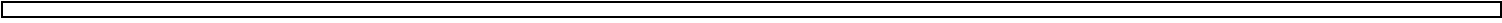
\includegraphics[width=.22\linewidth]{blank}%
\label{subfig:scribble-vis-image}}
\hfil
\subfloat[正确结果]{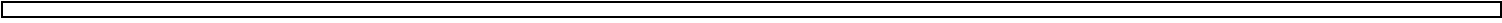
\includegraphics[width=.22\linewidth]{blank}%
\label{subfig:scribble-vis-gt}}
\hfil
\subfloat[涂鸦线标签]{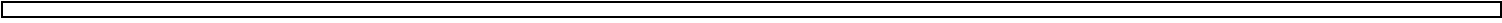
\includegraphics[width=.22\linewidth]{blank}%
\label{subfig:scribble-vis-label}}
\hfil
\subfloat[GAP-CAM 结果]{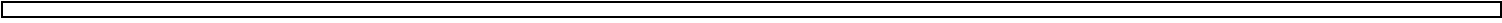
\includegraphics[width=.22\linewidth]{blank}%
\label{subfig:scribble-vis-gapcam}}
\caption{可视化}
\label{fig:scribble-vis}
\end{figure}

\subsection{针对 GAP-CAM 的消融实验}

\begin{table}[h]\label{tab:scribble-exp-pseudo}
\renewcommand{\arraystretch}{1.2}
\caption{伪标签质量消融实验}
\centering
\begin{tabular}{cccc|c}
\toprule[1.5pt]
涂鸦线标签 & 视觉注意力图 & 随机游走算法 & 条件随机场 & mIoU(\%) \\
\midrule[1.0pt]
$\sqrt{}$ &           &           &           & 20.00 \\
          & $\sqrt{}$ &           &           & 47.43 \\
$\sqrt{}$ & $\sqrt{}$ &           &           & 48.00 \\
$\sqrt{}$ & $\sqrt{}$ &           & $\sqrt{}$ & 52.40 \\
$\sqrt{}$ & $\sqrt{}$ & $\sqrt{}$ &           & 58.10 \\
$\sqrt{}$ & $\sqrt{}$ & $\sqrt{}$ & $\sqrt{}$ & 59.70 \\
\bottomrule[1.5pt]
\end{tabular}
\end{table}

\begin{table}[h]\label{tab:scribble-exp-pseudo}
\renewcommand{\arraystretch}{1.2}
\caption{相似度衡量标准}
\centering
\begin{tabular}{ccccc|c}
\toprule[1.5pt]
涂鸦线标签 & \makecell{超像素亮度\\均值距离} & 视觉注意力图 & \makecell{全连接网络\\相似性图} & \makecell{图卷积网络\\相似性图} & mIoU(\%) \\
\midrule[1.0pt]
$\sqrt{}$ &           &           &           &           &  \\
$\sqrt{}$ & $\sqrt{}$ &           &           &           &  \\
$\sqrt{}$ &           & $\sqrt{}$ &           &           &  \\
$\sqrt{}$ &           &           & $\sqrt{}$ &           &  \\
$\sqrt{}$ &           &           &           & $\sqrt{}$ &  \\
\bottomrule[1.5pt]
\end{tabular}
\end{table}

\begin{table}[h]\label{tab:scribble-exp-pseudo}
\renewcommand{\arraystretch}{1.2}
\caption{超像素生成算法消融实验}
\centering
\begin{tabular}{c|cc}
\toprule[1.5pt]
\diagbox{弱监督方法}{IoU}{超像素生成算法} & EGBIS & SLIC \\
\midrule[1.0pt]
ScribbleSup & 63.1 & ? \\
A$2$GNN & ? & 76.2 \\
GAP-CAM & ? & 76.5 \\
\bottomrule[1.5pt]
\end{tabular}
\end{table}

\subsection{针对 GAP-CAM 的超参数敏感性分析}

\begin{figure}[h]
\centering
\includegraphics[width=0.7\linewidth]{scribble-area}
\caption{涂鸦线长度比例}
\label{fig:scribble-area}
\end{figure}
% RTR tab1

\begin{figure}[h]
\centering
\includegraphics[width=.22\linewidth]{scribble-rw-image-1}
\hfil
\includegraphics[width=.22\linewidth]{scribble-rw-iter0-1}
\hfil
\includegraphics[width=.22\linewidth]{scribble-rw-iter1-1}
\hfil
\includegraphics[width=.22\linewidth]{scribble-rw-iter2-1}
\vfil
\includegraphics[width=.22\linewidth]{scribble-rw-image-2}
\hfil
\includegraphics[width=.22\linewidth]{scribble-rw-iter0-2}
\hfil
\includegraphics[width=.22\linewidth]{scribble-rw-iter1-2}
\hfil
\includegraphics[width=.22\linewidth]{scribble-rw-iter2-2}
\vfil
\includegraphics[width=.22\linewidth]{scribble-rw-image-3}
\hfil
\includegraphics[width=.22\linewidth]{scribble-rw-iter0-3}
\hfil
\includegraphics[width=.22\linewidth]{scribble-rw-iter1-3}
\hfil
\includegraphics[width=.22\linewidth]{scribble-rw-iter2-3}
\subfloat[输入图像]{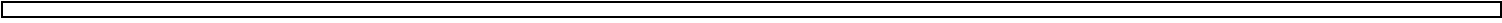
\includegraphics[width=.22\linewidth]{blank}%
\label{subfig:scribble-rw-image}}
\hfil
\subfloat[初始伪标签]{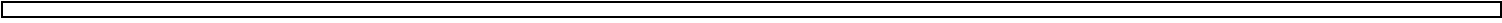
\includegraphics[width=.22\linewidth]{blank}%
\label{subfig:scribble-rw-iter0}}
\hfil
\subfloat[随机游走 128 轮]{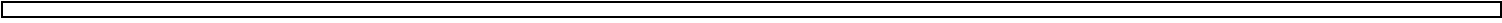
\includegraphics[width=.22\linewidth]{blank}%
\label{subfig:scribble-rw-iter1}}
\hfil
\subfloat[随机游走 256 轮]{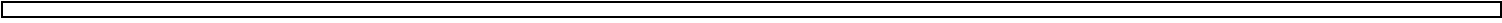
\includegraphics[width=.22\linewidth]{blank}%
\label{subfig:scribble-rw-iter2}}
\caption{可视化结果}
\label{fig:scribble-vis}
\end{figure}
% AE-PSL fig5
% 不能迭代过多否则溢出


不同迭代轮数伪标签曲线,加CRF(AE-PSL tab3,AffinityNet tab1)

CAM 成为可信像素的阈值 $\alpha$

哈达玛积轮数 $\alpha$

网格搜索(AffinityNet fig8fig9)

\section{本章小结}
一段话。
